\section{Ordinary differential equations}
\subsection{Definition}
\href{https://en.wikipedia.org/wiki/Ordinary_differential_equation}{An ODE} is a differential equation where it's derivatives belong to only one variable. Furthermore it is possible that an ODE can not be solved explicitly, due to that in this chapter it will be investigated how they can be solved numerically. \newline A first order differential value problem can be expressed like the one in \autoref{eq:first_order_problem}
\begin{equation}\label{eq:first_order_problem}
y^{\prime}(x)=f(x, y(x)) \text{  with initial condition  }y\left(x_0\right)=y_0
\end{equation}
\subsection{Explicit methods}
One way to solve the problem numerically is by \href{https://en.wikipedia.org/wiki/Taylor_series}{tailor series approximation}, as it can be seen in \autoref{eq:tailor_expansion}. (Remember that the tailor series is evaluated from one single point). The idea is that one creates a tailor series approximation up to order $p$ at the starting point and moves then with a step size $h$ to the new position one got from the tailor series approximation and does there the same until one reaches the destination.

\begin{multline}\label{eq:tailor_expansion}
y(x+h)= y(x)+\frac{y^{\prime}(x)}{1 !} h+\frac{y^{\prime \prime}(x)}{2 !} h^2+\frac{y^{\prime \prime \prime}(x)}{3 !} h^3 + \frac{y^{(4)}(x)}{4 !} h^4+\cdots+\frac{y^{(p)}(x)}{p !} h^p+\underbrace{\frac{y^{(p+1)}(\xi)}{(p+1) !} h^{p+1}}_{\text {remaining term}}
\end{multline}
The calculations up to order three (p=3) are given in \autoref{eq:tailor_expansion_formulas}:
\begin{equation}\label{eq:tailor_expansion_formulas}
\resizebox{.9\hsize}{!}{$
\begin{aligned}
y(x+h)= & y(x)+\frac{f(x, y(x))}{1 !} h+ \\
& \frac{1}{2 !}\left(\frac{\partial f(x, y(x))}{\partial x} 1+\frac{\partial f(x, y(x))}{\partial y} f(x, y(x))\right) h^2+ \\
& \frac{1}{3 !}\left(\frac{\partial^2 f(x, y(x))}{\partial x^2} 1+2 \frac{\partial^2 f(x, y(x))}{\partial x \partial y} f(x, y(x))+\frac{\partial^2 f(x, y(x))}{\partial y^2} f(x, y(x))^2+\left(\frac{\partial f(x, y(x))}{\partial y}\right)^2 f(x, y(x))+\frac{\partial f(x, y(x))}{\partial x} \frac{\partial f(x, y(x))}{\partial y}\right) h^3+\ldots+ \\
& \frac{1}{4 !} y^{(4)}(x) h^4+\ldots+\frac{1}{p !} y^{(p)}(x) h^p+\underbrace{\frac{1}{(p+1) !} y^{(p+1)}(\xi) h^{p+1}}_{\text {remaining term}}
\end{aligned}$}
\end{equation}
\subsubsection{Euler method}
The \href{https://en.wikipedia.org/wiki/Euler_method}{Euler method} is a special case of the explicit methods where $p=1$ and $h=const$. The Formulas to calculate it can be found in \autoref{eq:euler_method}.
\begin{equation}\label{eq:euler_method}
\begin{gathered}
y_0=y\left(x_0\right) \\
y\left(x_0+h\right) \approx y_1=y_0+f\left(x_0, y_0\right) h \approx y\left(x_0\right)+y^{\prime}\left(x_0\right) h \\
y\left(x_1+h\right) \approx y_2=y_1+f\left(x_1, y_1\right) h \approx y\left(x_1\right)+y^{\prime}\left(x_1\right) h \\
\vdots \\
y\left(x_{n-1}+h\right) \approx y_n=y_{n-1}+f\left(x_{n-1}, y_{n-1}\right) h \approx y\left(x_{n-1}\right)+y^{\prime}\left(x_{n-1}\right) h
\end{gathered}
\end{equation}
\subsubsection{Error Calculation}
\begin{itemize}
    \item \textbf{Global Error:} 
    \begin{equation}\label{eq:global_error_explicit_method}
    \max _{0 \leq i \leq k}\left|y_i-y\left(x_i\right)\right|
    \end{equation}
    \item \textbf{Local Error:}
    \begin{equation}\label{eq:local_error_explicit_method}
    y\left(x_n+h\right)-y_{n+1}= \underbrace{y(x+h)}_{\text{true output}}- \underbrace{(y(x)+y'(x)h)}_{\text{approx. output}}=h \cdot \tau_h\left(x_n\right)
    \end{equation}
     \item \textbf{Local slope Error:}
    \begin{equation}\label{eq:local_slope_error_explicit_method}
    \tau_h\left(x_n\right):=\frac{y\left(x_n+h\right)-y\left(x_n\right)}{h}-\left(\frac{y^{\prime}\left(x_n\right)}{1 !}+\frac{y^{\prime \prime}\left(x_n\right)}{2 !} h^1+\cdots \frac{y^{(p)}\left(x_n\right)}{p !} h^{p-1}\right)
    \end{equation}
\end{itemize}
\subsubsection{Example}
% The following example can not be solved easily, but one can calculate the derivative quite easily at each point and then draw a line that follows the derivatives.
% \begin{equation}
% \varphi^{\prime}(t)=2 \frac{a b \pi}{T} \frac{(1-\varepsilon \cos (\varphi(t)))^2}{p^2} \quad \varphi(0)=0
% \end{equation}
% The ellipse can also be expressed in the following way:
% \begin{equation}
% x=r(\varphi) \cos (\varphi), y=r(\varphi) \sin (\varphi)
% \end{equation}
% when we substitute, $c:=2 \frac{a b \pi}{T p^2}$ 
% one gets 
% \begin{equation}
% \varphi^{\prime}=c(1-\varepsilon \cos (\varphi))^2 \quad \varphi(0)=0
% \end{equation}
% When one now uses the Euler approximation one gets the following:
% $$
% \begin{aligned}
% &\varphi_0=0\\
% &\varphi_{k+1}=\varphi_{k+1}\cdot h\\
% \end{aligned}
% $$
% \paragraph{Errors}
% Global Error:
% Local Error ($T_h=\frac{y(x+h)-y(x)}{h}-\underbrace{\left(y'(x)\right)}_{\text{approx. slpe}}$): assumes that we start on a correct point. Local error does not want to know what happened in the past.
% $h \cdot T_h = \text{= absolute local error ('output')}= \underbrace{y(x+h)}_{\text{true output}}- \underbrace{(y(x)+y'(x)h)}_{\text{approx. output}}$

% Note: $C^{\circ}=$continuous

% \subsection{Extension of the Euler Scheme}
% At the exam only one value must be calculated!
% \subsubsection{Example one}
Solve the initial value problem $y^{\prime}=x y^{1 / 3} \text{ with }  y(1)=1$ numerically by the method of Taylor with order p = 4 and fixed step-size h = 0.1 for the x-values 1.1 and 1.2 (two steps). All final (!) results should be rounded to the 10th digit. Furthermore, compute the local error (slope) as well as the global error for the two steps. Note that the exact solution of the equation is given by \autoref{eq:exact_solution}.
\begin{equation}\label{eq:exact_solution}
y=\left(\frac{x^2+2}{3}\right)^{3 / 2}
\end{equation}\newline
To find out $x$ at $1.1$ one firstly needs to calculate the it's tailor series approximation at the starting point.
$$
\begin{aligned}
&x=1, y=1
&y_0=1 \\
&y_1= x y^{1 / 3}=1\\
&y_2=y^{1 / 3}+\frac{1}{3} x^2 y^{-1 / 3}=\frac{4}{3} \\
&y_3=x y^{-1 / 3}-\frac{1}{9} x^3 y^{-1}=\frac{8}{9} \\
&y_4=y^{-1 / 3}-\frac{2}{3} x^2 y^{-1}+\frac{1}{9} x^4 y^{-5 / 3}=\frac{4}{9} \\
\end{aligned}
$$
With \autoref{eq:tailor_expansion} one can then write down the following:
$$
\begin{aligned}
&y(1.1)= 1+\frac{1}{1 !} h+\frac{\frac{4}{3}}{2 !} h^2+\frac{\frac{8}{9}}{3 !} h^3+\frac{\frac{4}{9}}{4 !}=\underline{\underline{1.1068166666667}}\\
\end{aligned}
$$
Then one does the same at the new location on got from the previous result.

$$
\begin{aligned}
&x=1.1, &y=1.1068166666667\\
&y(1.2)=& y+\frac{x \cdot y^{1/3}}{1 !} h+\frac{y^{1 / 3}+\frac{1}{3} x^2 y^{-1 / 3}}{2 !} h^2+\frac{x y^{-1 / 3}-\frac{1}{9} x^3 y^{-1}}{3 !} h^3+\\&&\frac{y^{-1 / 3}-\frac{2}{3} x^2 y^{-1}+\frac{1}{9} x^4 y^{-5 / 3}}{4 !}=\underline{\underline{1.227872941753}}\\
\end{aligned}
$$
The global error is defined by \autoref{eq:global_error_explicit_method} and therefore has the following result:
$$
\begin{aligned}
& \max _{0 \leq i \leq 2}\left|y_i-y\left(x_i\right)\right|=\max \left\{\left|y_0-y\left(x_0\right)\right|,\left|y_1-y\left(x_1\right)\right|,\left|y_2-y\left(x_2\right)\right|\right\}= \\
& \max \left\{|1-1|,\left|y_1-\left(\frac{1.1^2+2}{3}\right)^{3 / 2}\right|,\left|y_2-\left(\frac{1.2^2+2}{3}\right)^{3 / 2}\right|\right\}=\underline{\underline{1.1473 \underline{4} \times 10^{-7}}}
\end{aligned}
$$
The local error is defined by \autoref{eq:local_slope_error_explicit_method} and therefore has the following result:
$$
\begin{aligned}
&n=0\\
& \tau_h\left(x_0\right):=\frac{y\left(x_0+h\right)-y\left(x_0\right)}{h}-\left(\frac{y^{\prime}\left(x_0\right)}{1 !}+\frac{y^{\prime \prime}\left(x_0\right)}{2 !} h^1+\cdots+\frac{y^{(4)}\left(x_0\right)}{4 !} h^{4-1}\right)= \\
& \frac{y(1.1)-y(1)}{h}-\left(\frac{y^{\prime}(1)}{1 !}+\frac{y^{\prime \prime}(1)}{2 !} h^1+\cdots+\frac{y^{(4)}(1)}{4 !} h^{4-1}\right)= \\
& \frac{\left(\frac{1.1^2+2}{3}\right)^{3 / 2}-\left(\frac{1^2+2}{3}\right)^{3 / 2}}{0.1}-\left(1+\frac{2}{3} 0.1+\frac{4}{27} 0.1^2+\frac{1}{54} 0.1^3\right)=\underline{\underline{-6.035828648 \times 10^{-7}}}
\end{aligned}
$$
and for n=1 one has the following result:
$$
\begin{gathered}
\tau_h\left(x_1\right):=\frac{y\left(x_1+h\right)-y\left(x_1\right)}{h}-\left(\frac{y^{\prime}\left(x_1\right)}{1 !}+\frac{y^{\prime \prime}\left(x_1\right)}{2 !} h^1+\cdots+\frac{y^{(4)}\left(x_1\right)}{4 !} h^{4-1}\right)= \\
\frac{y(1.2)-y(1.1)}{h}-\left(\frac{y^{\prime}(1.1)}{1 !}+\frac{y^{\prime \prime}(1.1)}{2 !} h^1+\cdots+\frac{y^{(4)}(1.1)}{4 !} h^{4-1}\right)= \\
\frac{\left(\frac{1.2^2+2}{3}\right)^{3 / 2}-\left(\frac{1.1^2+2}{3}\right)^{3 / 2}}{0.1}-(\ldots)=\underline{\underline{-5.2265445216 \times 10^{-7}}}
\end{gathered}
$$








\subsection{Explicit Runge-Kutta Methods}
Since the calculation of the tailor approximation series is quite tedious. One came up with another method, which is recursive and results in the same as the tailor series approximation (big advantage is that no computations of derivatives up to order p are needed). In \autoref{eq:common_runge_kutta_method} one can find the Common Runge-Kutta method of order 4. As one can see there one has seven variables, when one now sets this equal with the tailor series approximation all those variables are defined in the end as it can be seen in \autoref{eq:runge_kutta_method_types}.
\begin{equation}\label{eq:common_runge_kutta_method}
\begin{aligned}
& k_1=f(x, y) \\
& k_2=f\left(x+m h, y+m h k_1\right) \\
& k_3=f\left(x+n h, y+n h k_2\right) \\
& k_4=f\left(x+p h, y+p h k_3\right) \\
& y(x+h) \approx y(x)+a h k_1+b h k_2+c h k_3+d h k_4 \\
&
\end{aligned}
\end{equation}


\begin{equation}\label{eq:runge_kutta_method_types}
\begin{array}{lll}
\text {Name der Lösungen} & \# \text {Stages} $(s)$ & \text {Lösungen}\\
\hline
\text {Heun } & 2 & a=b=\frac{1}{2}, m=1(n=p=c=d=0) \\
\text {Explicit Midpoint } & 2 & a=0, b=1, m=\frac{1}{2}(n=p=c=d=0) \\
\text {Classic Runge-Kutta } & 4 & m=n=\frac{1}{2}, p=1, a=d=\frac{1}{6}, b=c=\frac{1}{3}
\end{array}
\end{equation}
% \begin{equation}
% \begin{aligned}
% & k_1=h f(x, y) \text { init (stages) } \\
% & k_2=h f\left(x+m h;y+m k_1\right).
% \end{aligned}
% \end{equation}
% \begin{equation}
% y(x+1 h) \approx y(x)+a k_1+b k_2
% \end{equation}
% The parameters are m, a, b \newline
% Simulate tailor up to order p=2
% \begin{equation}\label{eq:tailor_order_2}
% y(x+1 h) \approx y(x)+1h f+\frac{1}{2 !}(\underbrace{f_x+f_y f)}_{F_1} h^2
% \end{equation}
% \begin{equation}
% \left.\begin{array}{l}
% k_1=h f(x, y) \\
% k_2=h f\left(x+m h, y+m k_1\right)
% \end{array}\right\} \quad 2 \text { stages }
% \end{equation}
% Comparing \autoref{eq:tailor_order_2} with \autoref{eq:runge_kutta} one sees that a+b must be one and $bm=\frac{1}{2!}$
% \begin{equation}\label{eq:runge_kutta}
% y(x+h) \approx y(x)+(a+b) h f+(b m) F_1 h^2
% \end{equation}
% \begin{equation}
% y(x+h) \approx y(x)+\frac{1}{2} h f(x, y)+\frac{1}{2} h f(x+1 h, y+1 h f(x, y)) .
% \end{equation}
For the classic runge-kutta method one can also write \autoref{eq:common_runge_kutta_method_classic} which results in \autoref{eq:runge_kutta_k}.
\begin{equation}\label{eq:common_runge_kutta_method_classic}
\begin{aligned}
& k_1=h f(x, y) \\
& k_2=h f\left(x+m h, y+m k_1\right) \\
& k_3=h f\left(x+n h, y+n k_2\right) \\
& k_4=h f\left(x+p h, y+p k_3\right) \\
& y(x+h) \approx y(x)+a k_1+b k_2+c k_3+d k_4
\end{aligned}
\end{equation}
% $k_1$ is always the same the slope of the vector field times h. With order four one has seven degree of freedom and therefore 8 equations.\newline
% RK4 solution
% \begin{equation}
% m=n=\frac{1}{2}, \quad p=1, \quad a=d=\frac{1}{6}, \quad b=c=\frac{1}{3}
% \end{equation}
\begin{equation}\label{eq:runge_kutta_k}
\begin{aligned}
& k_1=h f(x, y) \\
& k_2=h f\left(x+\frac{1}{2} h, y+\frac{1}{2} k_1\right) \\
& k_3=h f\left(x+\frac{1}{2} h, y+\frac{1}{2} k_2\right) \\
& k_4=h f\left(x+h, y+k_3\right) \\
& y(x+h) \approx y(x)+\frac{1}{6}\left(k_1+2 k_2+2 k_3+k_4\right)
\end{aligned}
\end{equation}


The errors are calculated nearly the same way as in the previous section. \autoref{eq:runge_kutta_local_slope_error}.

\begin{itemize}
    \item \textbf{Global Error:} 
    \begin{equation}\label{eq:runge_kutta_global_error_explicit_method}
    \max _{0 \leq i \leq k}\left|y_i-y\left(x_i\right)\right|
    \end{equation}
    \item \textbf{Local Error:}
    \begin{equation}\label{eq:runge_kutta_local_error_explicit_method}
    h \cdot \tau_h\left(x_n\right)
    \end{equation}
    When there is only one step calculated, the local error must be the same as the global error.
    \item \textbf{Local slope Error:}
    \begin{equation}\label{eq:runge_kutta_local_slope_error}
    \tau_h\left(x_n\right):=\frac{y\left(x_n+h\right)-y\left(x_n\right)}{h}-\left(\sum_{j=1}^s b_j k_j\right)
    \end{equation}
\end{itemize}
\subsubsection{Example}
Solve the initial value problem $y^{\prime}=x y^{1 / 3} \quad y(1)=1$ numerically by the classical Runge-Kutta method of order p = 4 and fixed step-size h = 0.1 for the x-values 1.1 und 1.2 (two steps). All final (!) results should be rounded to the 10th digit. The exact solution of the equation is $y=\left(\frac{x^2+2}{3}\right)^{3 / 2}$.\newline
From \autoref{eq:runge_kutta_k} one knows that:
$$
\begin{aligned}
& k_1=h f(x, y)=h x y^{1 / 3} = 0.1\cdot 1 \cdot 1^{1/3}=0.1 \\
& k_2=h f\left(x+\frac{1}{2} h, y+\frac{1}{2} k_1\right)=0.1\cdot (1+\frac{1}{2}\cdot 0.1)\cdot (1+\frac{1}{2}\cdot 0.1)^{1/3}=0.10672161746556 \\
& k_3=h f\left(x+\frac{1}{2} h, y+\frac{1}{2} k_2\right)= 0.1\cdot (1+\frac{1}{2}\cdot 0.1)\cdot (1+\frac{1}{2}\cdot 0.10672161746556)^{1/3}=0.10683535998891 \\
& k_4=h f\left(x+h, y+k_3\right)=0.1 \cdot (1+0.1)\cdot (1+0.10683535998891)^{1/3}=0.11378552740653 \\
& y(x+h) \approx y(x)+\frac{1}{6}\left(k_1+2 k_2+2 k_3+k_4\right)=\underline{\underline{1.1068165803859}}
\end{aligned}
$$

$$
\begin{aligned}
& k_1=h f(x, y)=h x y^{1 / 3} = 0.1\cdot 1.1 \cdot 1.1068165803859^{1/3}=0.11378488387236 \\
& k_2=h f\left(x+\frac{1}{2} h, y+\frac{1}{2} k_1\right)=0.1\cdot (1+\frac{1}{2}\cdot 0.1)\cdot (1.1+\frac{1}{2}\cdot 0.11378488387236)^{1/3}=0.12096116868214 \\
& k_3=h f\left(x+\frac{1}{2} h, y+\frac{1}{2} k_2\right)= 0.1\cdot (1+\frac{1}{2}\cdot 0.1)\cdot (1.1+\frac{1}{2}\cdot 0.12096116868214)^{1/3}=0.12108536369591 \\
& k_4=h f\left(x+h, y+k_3\right)=0.1 \cdot (1.1+0.1)\cdot (1.1068165803859+0.12108536369591)^{1/3}=0.1284998068981 \\
& y(x+h) \approx y(x)+\frac{1}{6}\left(k_1+2 k_2+2 k_3+k_4\right)=\underline{\underline{1.2278795396403}}
\end{aligned}
$$
As one can see, the result is nearly the same as in the previous Example. The \textbf{local slope error} can be calculated according to \autoref{eq:runge_kutta_local_slope_error}.
$$
\begin{aligned}
& \tau_h\left(x_0\right):=\frac{y\left(x_0+h\right)-y\left(x_0\right)}{h}-\left(\frac{\tilde{k}_1+2 \tilde{k}_2+2 \tilde{k}_3+\tilde{k}_4}{6 h}\right)= \\
& \frac{\left(\frac{1.1^2+2}{3}\right)^{3 / 2}-\left(\frac{1^2+2}{3}\right)^{3 / 2}}{0.1}-\left(\frac{\tilde{k}_1+2 \tilde{k}_2+2 \tilde{k}_3+\tilde{k}_4}{0.6}\right)=\underline{\underline{2.5922467994 \times 10^{-7}}}
\end{aligned}
$$
$$
\begin{aligned}
& \tau_h\left(x_1\right):=\frac{y\left(x_1+h\right)-y\left(x_1\right)}{h}-\left(\frac{\tilde{k}_1+2 \tilde{k}_2+2 \tilde{k}_3+\tilde{k}_4}{6 h}\right)= \\
& \frac{\left(\frac{1.2^2+2}{3}\right)^{3 / 2}-\left(\frac{1.1^2+2}{3}\right)^{3 / 2}}{0.1}-\left(\frac{\tilde{k}_1+2 \tilde{k}_2+2 \tilde{k}_3+\tilde{k}_4}{0.6}\right)=\underline{\underline{2.7090772847 \times 10^{-7}}}
\end{aligned}
$$
The local error can be calculated according to \autoref{eq:runge_kutta_local_error_explicit_method} and results in the following:
$$
h \cdot \tau_h\left(x_0\right)=\underline{\underline{2.5922467994 \times 10^{-8}}}
$$
$$
h \cdot \tau_h\left(x_1\right)=\underline{\underline{2.7090772847 \times 10^{-8}}}
$$


% \subsection{Ex1.5}
% \begin{equation}
% \varphi^{\prime}=c(1-\xi \cos \varphi)^2 ; \varphi(0)=0=\varphi_0
% \end{equation}
% $$
% \begin{aligned}
% & k_1=h c(1-\xi \cos \varphi)^2 \\
% & k_2=h c(1-\xi \cos(\varphi_k+\frac{1}{2}k_1) )^2 \\
% & k_3=h c(1-\xi \cos(\varphi_k+\frac{1}{2}k_2) )^2 \\
% & k_3=h c(1-\xi \cos(\varphi_k+1 k_3) )^2 \\
% & y(k+1) = y_k+\frac{1}{6}\left(k_1+2 k_2+2 k_3+k_4\right)
% \end{aligned}
% $$

\subsection{Butcher tableau}
The \href{https://en.wikipedia.org/wiki/Runge%E2%80%93Kutta_methods}{Butcher tableau} is mainly a mnemonic device (Gedächtnissstütze) to remember the coefficients. The tableau must fullfill the condition listed in \autoref{con:butcher_tableau}
\begin{equation}\label{con:butcher_tableau}
\begin{aligned}
& c_i=\sum_{j=1}^s a_{i j}=\sum_{j=1}^{i-1} a_{i j}(i=2, \ldots, s) \\
& \sum_{j=1}^s b_j=1 \\
& c_1=0 \\
& a_{1 j}=0 \quad 1 \leq j \leq s \\
& a_{i j}=0 \quad j \geq i \\
&
\end{aligned}
\end{equation}
Where the variables mean the folwoing:
\begin{itemize}
    \item s= number of stages
    \item c= 'inputs' Subdivides inputs
    \item b= weights
    \item a = subdiv 'y' 'output'
\end{itemize}
The general tableau can be seen in \autoref{eq:butcher_tableau_normal}.
\begin{equation}\label{eq:butcher_tableau_normal}
\begin{array}{c|cccc}
 & k_1 & k_2 & \dots & k_S\\
\hline 
c_1 & a_{11} & a_{12} & \dots & a_{1s}\\
c_2 & a_{21} & a_{22} & \dots & a_{2s}\\
\vdots & \vdots & \vdots & & \vdots \\
c_s & a_{S1} & a_{S2} & \dots & a_{ss}\\
\hline
&b_1&b_2 & \dots & b_S
\end{array}
\end{equation}
A step from $x_n$ to $x_{n+1}=x_n+h_n (n=0,1,\dots)$ in the general Runge-Kutta method is defined by \autoref{eq:general_runge_kutta} where the values $a,b,c$ can be read from the butcher tableau.
\begin{equation}\label{eq:general_runge_kutta}
\begin{array}{l}
\left.\begin{array}{l}
k_1=f\left(x_n+c_1 h_n, y_n+h_n \sum_{j=1}^s a_{1, j} k_j\right) \\
k_2=f(x_n+c_2 h_n, \underbrace{y_n+h_n \sum_{j=1}^s a_{2, j} k_j}_{g_2}) \\
k_3=f(x_n+c_3 h_n, \underbrace{y_n+h_n \sum_{j=1}^s a_{3, j} k_j}_{g_3}) \\
\vdots \\
k_s=f(x_n+c_s h_n, \underbrace{y_n+h_n \sum_{j=1}^s a_{s, j} k_j}_{g_s})
\end{array}\right\} \text{s stages}\\ \\
y_{n+1}=y_n+h_n \sum_{j=1}^s b_j k_j
\end{array}
\end{equation}
Some examples for butcher tableaus can be found in \autoref{table:butcher_tableaus}
\begin{table}[ht]
  \centering
  \resizebox{1\textwidth}{!}{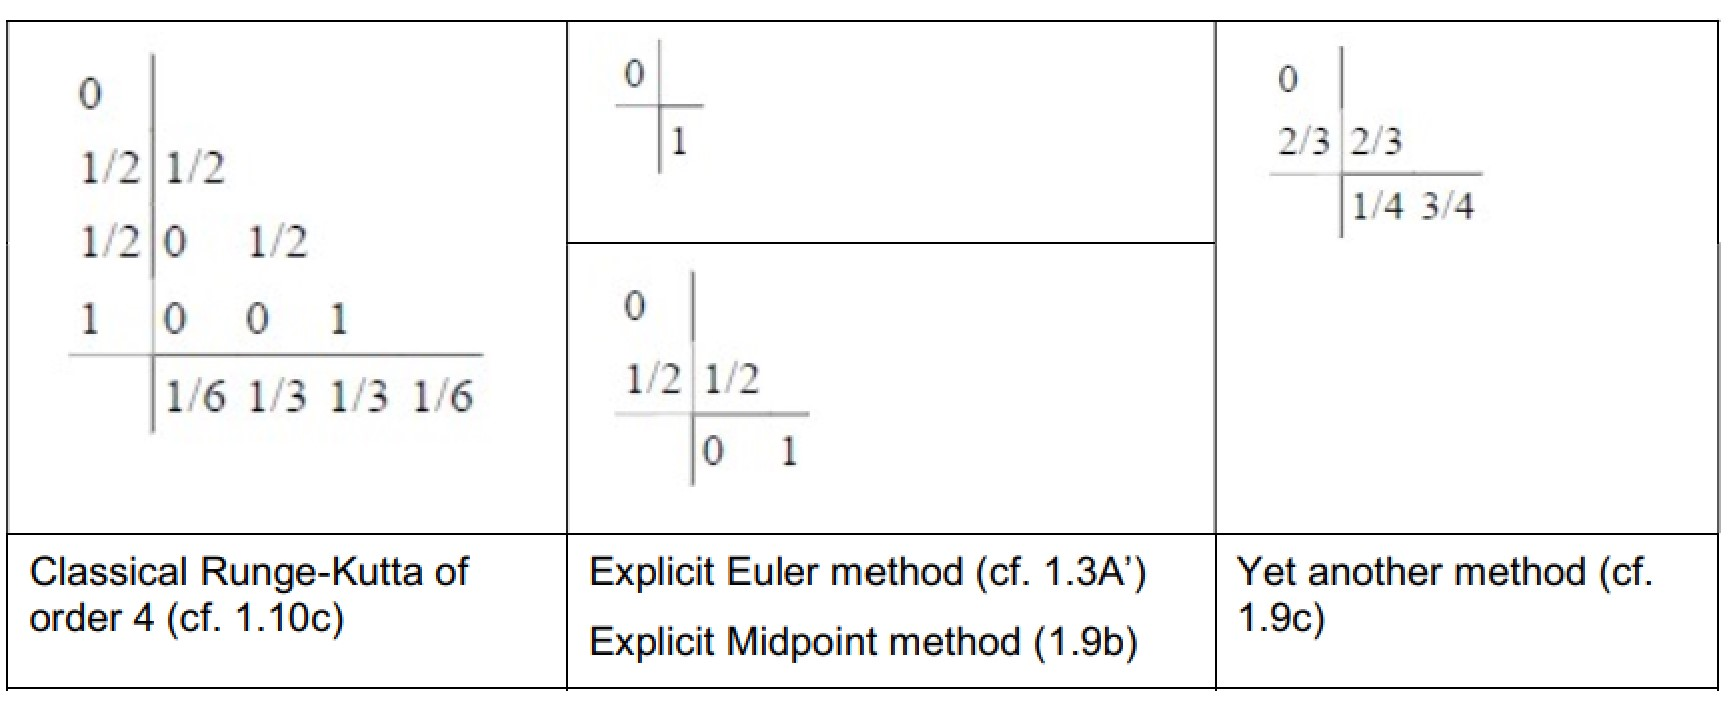
\includegraphics{images/butcher_tableaus.jpg}}
  \caption{Butcher Tableaus}
  \label{table:butcher_tableaus}
\end{table}\newline
\href{https://en.wikipedia.org/wiki/List_of_Runge%E2%80%93Kutta_methods}{The simplest adaptive Runge–Kutta method involves combining Heun's method, which is order 2, with the Euler method, which is order 1} (also called Heun-Euler 2(1)). Its extended Butcher Tableau can be seen in \autoref{eq:heun_euler_2_1}. 
\begin{equation}\label{eq:heun_euler_2_1}
\begin{array}{c|cc}
0 & & \\
1 & 1 & \\
\hline & 1 / 2 & 1 / 2 \\
& 1 & 0
\end{array}
\end{equation}

\subsection{Step-size adaption}
\subsubsection{Idea}
The Idea is to automatically adapt the step-size $h$. Due to that one needs a new way to define the approximation of the error, which can be done with an Accuracy Goal $(ac)$, which defines how many decimal places (Nachkommastellen) are correct and a precision Goal $(pg)$, which represents the significant digits of the result. The two parameters are considered in the tolerance parameter, $\varepsilon$ which can be found in \autoref{eq:tolerance_parameter}.
\begin{equation}\label{eq:tolerance_parameter}
    \varepsilon=\varepsilon_{a}+|y| \varepsilon_{r}=10^{-a g}+|y| 10^{-p g} \geq|e|
\end{equation}
Furthermore, one needs a second approximation for the error calculation, with the order $\hat{p}$. The first order approximation $p$ is needed to calculate the step size. Mostly $\hat{p}=p-1$. Due to that the butcher tableau is extended by a row ($b$ values) as it can be seen in \autoref{table:butcher_2}.
\begin{table}[ht]
\centering
\begin{tabular}{|c|ccccc|}
\hline 0 & 0 & 0 & $\cdots$ & 0 & 0 \\
$c_{2}$ & $a_{2,1}$ & 0 & $\cdots$ & 0 & 0 \\
$\vdots$ & $\vdots$ & $\vdots$ & $\ddots$ & 0 & $\vdots$ \\
$c_{s-1}$ & $a_{s-1,1}$ & $a_{s-1,2}$ & $\cdots$ & 0 & 0 \\
$c_{s}$ & $a_{s, 1}$ & $a_{s, 2}$ & $\cdots$ & $a_{s, s-1}$ & 0 \\
\hline & $b_{1}$ & $b_{2}$ & $\cdots$ & $b_{s-1}$ & $b_{s}$ \\
& $\hat{b}_{1}$ & $\hat{b}_{2}$ & $\cdots$ & $\hat{b}_{s-1}$ & $\hat{b}_{s}$ \\
\hline
\end{tabular}
\caption{Butcher Table}
\label{table:butcher_2}
\end{table}
The local error can be calculated according to \autoref{eq:adaptive_local_error}.
\begin{equation}\label{eq:adaptive_local_error}
    e_{n}=y(x+h)-\hat{y}(x+h)=h_{n} \sum_{j=1}^{s}\left(b_{j}-\hat{b}_{j}\right) k_{j} \Rightarrow\left\|e_{n}\right\|=\left\|h_{n} \sum_{j=1}^{s}\left(b_{j}-\hat{b}_{j}\right) k_{j}\right\|
\end{equation}
Below one can find again a short description of the variables:
\begin{itemize}
    \item $\varepsilon_{a}=dy$: absolute error $\varepsilon_{a}=10^{-ag}$ \newline
    Ex. $ag=4 \Rightarrow 0.\textcolor{red}{0012}89$
    \item $\varepsilon_{r}=\frac{dy}{y\ne 0}$: relative error $\varepsilon_{r}=10^{-pg}$\newline
    Ex. $pg=4 \Rightarrow 0.00\underbrace{\textcolor{red}{1289}}_{\text{signific. digit}}$
\end{itemize}


To know if the step size is good or not one calculates $\frac{\left\|e_{n}\right\|}{\varepsilon}$. When the current step $\frac{\left\|e_{n}\right\|}{\varepsilon}>1$, then the estimation of $h_{n}$ was too optimistic and the step must be repeated with a smaller step size. One also says the current step is \textbf{Rejected}. Otherwise when $\frac{\left\|e_{n}\right\|}{\varepsilon}\leq 1$ the step size is ok and one can \textbf{proceed}.
Updating the step size is done according to \autoref{eq:step_size}.
\begin{equation}\label{eq:step_size}
    h_{n+1}=h_{n}\left(\frac{\varepsilon}{\left\|e_{n}\right\|}\right)^{\frac{1}{\bar{p}}}=h_{n}\left(\frac{\left\|e_{n}\right\|}{\varepsilon}\right)^{-\frac{1}{\bar{p}}}
\end{equation}
$\varepsilon=\varepsilon_{a}+\varepsilon_{r}\left|y_{n}\right| \quad$ with $\quad \tilde{p}=\min (p, \hat{p})+1$ (order of the primary method)


\subsubsection{Stability of explicit methods}
The global relative error must not diverge, which means it must be limited. Since it is difficult to make a statement about the analysed ODE one uses benchmark equations. One of the most commonly used ones is the Dahlquist model, which can be seen in \autoref{eq:dahlquist}
\begin{equation}\label{eq:dahlquist}
    y^{\prime}=A y \quad y(0)=1 \quad \text { mit } A=\Re\{A\}+j \Im\{A\} \in \mathbb{C}
\end{equation}
The solution of this equation is $y=e^{\Re\{A\} x}\left(\cos (\Im\{A\} x+j \sin (\Im\{A\} x))\right.$, which is an oscillation with a exponential amplitude $e^{\Re\{A\} x}$ and  frequency $\Im\{A\}$. The 
\paragraph{Example Euler}
$$
Y^{\prime}=-\lambda Y ; Y(0)=1 ; x \geq 0 ; \lambda>0
$$
The exact solution is: $\quad Y(x)=e^{-\lambda x}$
Consider Euler's method: Solation will go to zero iff
$$
\begin{aligned}
y_{n+1} & =y_n+h f\left(x_n, y_n\right) & & |1-h \lambda|<1 \Rightarrow \frac{2}{\lambda}>h>0 \\
& =y_n-h \lambda y_n & & \text { Euler's method is stable for } \\
& =(1-h \lambda) y_n & & \text { this ODE if } \quad 0<h<\frac{2}{\lambda}
\end{aligned}
$$
\paragraph{Stability for heun-method (rk-2)}\mbox{}\newline
From \autoref{eq:general_runge_kutta} one knows that $y_{k+1}=y_k+h\cdot (\frac{1}{2}\cdot k_1+\frac{1}{2}\cdot k_2)$
\begin{equation}
\begin{array}{lc}
k_{1}=A y_{k} & y_{0}=y\left(x_{0}\right)=y(0)=1 \\
k_{2}=A\left(y_{k}+1 h k_{1}\right)=A\left(y_{k}+A h y_{k}\right) \quad \Longrightarrow \quad &y_{k+1}=y_{k} \underbrace{\left(1+h A+(h A)^{2} \frac{1}{2}\right)}_{F(h A)=F(z), \quad z=h A \in \mathbb{C}}
\end{array}
\end{equation}
From that one can somehow derive three cases which are listed below


\paragraph{3 Cases}
\begin{itemize}
    \item $\Re\{A\}<0$: The Amplitude of the ODE gets smaller exponentially. The stability conditions says that the approximated values $y_{k}(k=0,1, \ldots)$ must be exponentially damped too. Therefore and from $y_{k+1} \propto|F(z)|$ the following must hold $|F(z)|<1$.
    \item $\Re\{A\}=0$ : The Amplitude of the ODE is constant. The stability conditions says that the approximated values $y_{k}(k=0,1, \ldots)$ are constant too. Therefore and from $y_{k+1} \propto|F(z)|$ the following must hold $|F(z)|=1$.
    \item $\Re\{A\}>0$ : The Amplitude of the ODE gets larger exponentially. The stability conditions says that the approximated values $y_{k}(k=0,1, \ldots)$ must be exponentially growing too. Therefore and from $y_{k+1} \propto|F(z)|$ the following must hold $|F(z)|>1$.
\end{itemize}
The stability condition for case one can know be calculated as the following $(\Re\{A\}<0)$ and $1>|F(z)|=\left|1+h A+\frac{1}{2}(h A)^{2}\right| \Rightarrow-2<h \Re\{A\}<0$.  since $x_{1,2}=\frac{-b \pm \sqrt{(b^2-4\cdot a \cdot c)}}{2 \cdot a}=\frac{-1 \pm \sqrt{((1)^2-4\cdot 0 \cdot \frac{1}{2})}}{2 \cdot \frac{1}{2}}=-1 \pm 1$ and therefore the values must be between 0 and -2. The \textbf{stability polynomial} in this exercise was $F(z)=1+z+\frac{z^2}{2} \quad(z=h A)$.
\paragraph{Recursive Formulas}\mbox{}\newline
For the stability polynomials in the form: $F(z)=1+b_{1} k_{1}(z)+\ldots+b_{s} k_{s}(z)$ recursive equations exist as can be seen in \autoref{eq:recursive_formula}.
\begin{equation}\label{eq:recursive_formula}
 k_{1}(z)=z, \quad k_{j+1}(z)=z\left(1+a_{j+1,1} k_{1}(z)+a_{j+1,2} k_{2}(z)+\ldots+a_{j+1, j} k_{j}(z)\right)
\end{equation}
\subsubsection{Exercise adaptive step size}
Solve the initial value problem $\varphi^{\prime}=c(1-\varepsilon \cos \varphi)^2 \quad \varphi(0)=0$ with $c=1$ and $\epsilon=0.25$ numerically by applying the Heun-Euler 2(1) embedded adaptive method with classical step-size control until 3 proceeding steps are executed. The initial step-size equals $0.001$, the accuracy goal (ag) 4 and the precision goal is 4 , either.\newline
Create a table listing values for $\left(x, y, h, e_k,\left(\frac{\left\|e_k\right\|}{\varepsilon}\right)^{-\frac{1}{\widetilde{p}}}, h_{\text {new }}\right.$, state $)$ containing at least three preceding steps.\newline 
According to the exercise, we know the following:
\begin{enumerate}
    \item The position at the beginning: $x=0$, $y=0$
    \item The step size: $h=0.001$
    \item The local error can be calculated according to \autoref{eq:adaptive_local_error}. Which says that $e_{k}=h_{n} \sum_{j=1}^{s}\left(b_{j}-\hat{b}_{j}\right) k_{j}$. From \autoref{eq:heun_euler_2_1} one knows $b_1=\frac{1}{2}$, $\hat{b}_1=1$, $b_2=\frac{1}{2}$ and $\hat{b}_2=0$. Furthermore, one knows from \autoref{eq:general_runge_kutta} and \autoref{eq:heun_euler_2_1} that $k_1=f\left(x_n+\underbrace{0}_{c_1}\cdot h_n, y_n+h_n\cdot \underbrace{0}_{a_{1,j}} \right)=1\cdot \left(1-\frac{1}{4} \cos{0}\right)^2=\textcolor{blue}{\frac{9}{16}}$ and 
    $k_2=f\left(x_n\textcolor{gray}{+\underbrace{\xout{1}}_{c_2}\cdot \xout{h_n}}, y_n+h_n\cdot \underbrace{1}_{a_{2,1}}\cdot k_1\right)=1 \cdot \left(1-(\frac{1}{4}\cdot \cos{(0.001\cdot 1 \cdot \textcolor{blue}{\frac{9}{16}})}\right)^2=\textcolor{orange}{0.5625}$. Therefore $e_k=h_n\cdot (b_1-\hat{b}_1)\cdot k_1+(b_2-\hat{b}_2)\cdot k_2=\underbrace{0.001}_{h_n}\cdot (\underbrace{-\frac{1}{2}}_{b_1-\hat{b}_1}\cdot\textcolor{blue}{\frac{9}{16}} + \underbrace{\frac{1}{2}}_{(b_2-\hat{b}_2)} \cdot \textcolor{orange}{0.5625} )= \textcolor{brown}{2.966\cdot 10^{-11}}$
    \item Since $p=2$ (order) and $\varepsilon$ can be calculated according to \autoref{eq:tolerance_parameter} which says: $\varepsilon=\varepsilon_{a}+|y| \varepsilon_{r}=10^{-a g}+|y| 10^{-p g} = 10^{-4}+0 \cdot  10^{-4}=10^{-4}$. Therefore $\left(\frac{\left\|e_k\right\|}{\varepsilon}\right)^{-\frac{1}{\widetilde{p}}}=\left(\frac{\textcolor{brown}{2.966\cdot 10^{-11}}}{10^{-4}}\right)^{-\frac{1}{2}}=1.836\cdot 10^3$
    \item With \autoref{eq:step_size} one can the finally calculate the new step size which is: $h_{n+1}=h_{n}\left(\frac{\left\|e_{n}\right\|}{\varepsilon}\right)^{-\frac{1}{\bar{p}}}=0.001\cdot \left(\frac{\textcolor{brown}{2.966\cdot 10^{-11}}}{10^{-4}}\right)^{-\frac{1}{2}}=1.836$
    \item the new y value can be calculated according to \autoref{eq:general_runge_kutta} which means for the current scheme $0.001\cdot (\frac{1}{2}\cdot k_1+\frac{1}{2}\cdot k_2)=0.001\cdot (\frac{1}{2}\cdot \textcolor{blue}{\frac{9}{16}}+\frac{1}{2}\cdot \textcolor{orange}{0.5625})=0.0005625$
\end{enumerate}

\begin{table}[ht]
    \centering
    \begin{tabular}{|c|c|c|c|c|c|c|}
    \hline x & y &  $h_n$ & $e_k$ & $\left(\frac{\left\|e_k\right\|}{\varepsilon}\right)^{-\frac{1}{\widetilde{p}}}$ & $h_{n+1}$&state\\
    \hline
    0& 0& 0.001 &$\textcolor{brown}{2.966\cdot 10^{-11}}$&$1.836\cdot 10^3$&1.836&Proceed\\
    \hline
    0.001& 0.0005625&1.836&0.18169&0.02347&0.043&Reject\\
    \hline
    \end{tabular}
    \caption{Exercise}
    \label{tab:example_tab}
\end{table}

\subsubsection{Exercise Stability polynomial}
Using Theorem $1.3$ in the script (p. 29) gain the A-stability polynomial $F_1(z)=1+z+\frac{z^2}{2}+\frac{z^3}{6}$ for the embedded adaptive method SS3(2) with Butcher tableau.
$$
\begin{array}{c|cccc}
0\\
\frac{1}{2} & \textcolor{orange}{\frac{1}{2}} & & \\
1 & \textcolor{brown}{-1} & \textcolor{blue}{2} &  \\
1 &  \frac{1}{6} & \frac{2}{3} & \frac{1}{6} \\
\hline
&\textcolor{pink}{\frac{1}{6}} & \textcolor{purple}{\frac{2}{3}} & \frac{1}{6}&0 \\
&\frac{1}{72}(\sqrt{82}-10) & \frac{1}{36}(10-\sqrt{82}) & \frac{1}{144}(28-\sqrt{82}) & \frac{1}{48}(\sqrt{82}-16)
\end{array}
$$
From \autoref{eq:recursive_formula} one knows that a stability polynomial is of the form $F(z)=1+b_1 k_1(z)+b_2 k_2(z)+b_3 k_3(z)+0 k_4(z)$, whereas:
$$
\begin{aligned}
& k_1(z)=z \\
& k_2(z)=z\left(1+\textcolor{orange}{\frac{1}{2}} k_1(z)\right)=z\left(1+\frac{1}{2} z\right) \\
& k_3(z)=z\left(1+\textcolor{brown}{-1} k_1(z)+\textcolor{blue}{2} k_2(z)\right)=z\left(1-z+2 z\left(1+\frac{1}{2} z\right)\right)=z+z^2+z^3
\end{aligned}
$$
$$
\text { Therefore } F(z)=1+\textcolor{pink}{\frac{1}{6}} k_1(z)+\textcolor{purple}{\frac{2}{3}} k_2(z)+\frac{1}{6} k_3(z)=1+z+\frac{1}{2} z^2+\frac{1}{6} z^3
$$
\subsubsection{Stiffness}\label{subsubsec:stiffnes}

The stiffnes is dependent on:
\begin{itemize}
    \item ODE
    \item step size h
    \item Method (for example RK-4)
\end{itemize}
\paragraph{Stiffness Detection}\mbox{}\newline
Heun euler does not work when we have stiffness situations.
Condition: $c_{s-1}=c_{s}=1$. Through testing of $\left|h \frac{\partial f(x, y)}{\partial y}\right|$ to the absolute borders of the stability region the stiffness can be detected. Stiffness is present when $|h \tilde{\lambda}|$ is outside or at the border of the stability condition.

\paragraph{Example for explicit runge-kutta}\mbox{}\newline
$$
k_{s-1}=f(x+c_{s-1} h, \underbrace{y+h \sum_{j=1}^{s} a_{s-1, j} k_{j}}_{g_{s-1}}) \quad k_{s}=f(x+c_{s} h, \underbrace{\left.y+h \sum_{j=1}^{s} a_{s, j} k_{j}\right)}_{g_{s}} \quad \Rightarrow \quad \tilde{\lambda}=\frac{\left\|k_{s}-k_{s-1}\right\|}{\left\|g_{s}-g_{s-1}\right\|}
$$
$\tilde{\lambda}$ is an estimation for $f_{y}=\frac{\partial}{\partial y} f(x, y)$ for example $y^{\prime}=x^{4}-25 y^{4}=f(x, y)$ and takes the role of $\Re\{A\}$ for the stability analysis.




\subsubsection{Exercise stiffness detection test}
Given the differential equation $y^{\prime}=\underbrace{-\sqrt{x^2+y^2}}_{f(x, y)} \quad y(0)=4 \quad$ carry out a stiffness detection test using the A-stability region and the partial derivative $f_y$ at the initial values and step size $h=1$. The method is defined by the Butcher tableau below.
$$
\begin{array}{l|ll}
0 & & \\
1 / 2 & \textcolor{orange}{1 / 2} & \\
b & \textcolor{pink}{0} & \textcolor{purple}{1} \\
\hat{b} & 1 & 0 \\
\hline
\end{array}
$$
The exercise can be solved in two steps:
\begin{enumerate}
    \item Get stability region (\autoref{eq:recursive_formula}):\newline
    From \autoref{eq:recursive_formula} one knows that a stability polynomial is of the form $F(z)=1+b_1 k_1(z)+b_2 k_2(z)+b_3 k_3(z)+0 k_4(z)$, whereas:
    $$
    \begin{aligned}
    & k_1(z)=z \\
    & k_2(z)=z\left(1+\textcolor{orange}{\frac{1}{2}} k_1(z)\right)=z\left(1+\frac{1}{2} z\right) \\
    \end{aligned}
    $$
    $$
    \text { Therefore } F(z)=1+\textcolor{pink}{0} k_1(z)+\textcolor{purple}{1} k_2(z)=1+z+\frac{1}{2} z^2 \text{ where } (z=h\cdot A)
    $$
    To calculate the stability region one hast to set the stability polynomial to zero and therefore one gets: $x_{1,2}=\frac{-b \pm \sqrt{(b^2-4\cdot a \cdot c)}}{2 \cdot a}=\frac{-1 \pm \sqrt{((1)^2-4\cdot 0 \cdot \frac{1}{2})}}{2 \cdot \frac{1}{2}}=-1 \pm 1$ and therefore the boundary is -2 and 0.
    \item Check stiffness (see \autoref{subsubsec:stiffnes})\newline
     By calculating the partial derivative of $-\sqrt{x^2+y^2}$ after y one obtains the following $-1\cdot \frac{1}{2}\cdot \frac{1}{\sqrt{x^2+y^2}} \cdot 2 \cdot y$ inserting $x=0$ and $y=4$ results in  $-1\Rightarrow A=-1$ and $h\cdot A =-1$ which is inside the A-stability constraint $-2<Ah<0$ and therefore no stiffness is detected.
\end{enumerate}

\subsubsection{Van der Pol second-order differential equation}
Solve the van-der-Pol ODE-system $\left(\begin{array}{l}z^{\prime}=v \\ v^{\prime}=\mu\left(1-z^2\right) v-z\end{array}\right) \quad z(0)=1, v(0)=-1, \quad \mu=0.2$ numerically by applying the Heun-Euler 2(1) embedded adaptive method with classical step-size control until 3 proceeding steps are executed. The initial step-size equals $0.001$, the accuracy goal (ag) 1 and the precision goal is 2.
Create a table listing values for $\left(t,\{z, v\}, h, e_k,\left\|\frac{\vec{e}_n}{\varepsilon_a+\varepsilon_r \vec{y}_n}\right\|^{-1 / \tilde{p}}, h_{\text {new, }}\right.$ state) containing at least three proceeding steps.

According to the exercise, we know the following:
\begin{enumerate}
    \item The position at the beginning: $x=0$, $z=0, v=-1$
    \item The step size: $h=0.001$
    \item The local error can be calculated according to \autoref{eq:adaptive_local_error}. Which says that $e_{k}=h_{n} \sum_{j=1}^{s}\left(b_{j}-\hat{b}_{j}\right) k_{j}$. From \autoref{eq:heun_euler_2_1} one knows $b_1=\frac{1}{2}$, $\hat{b}_1=1$, $b_2=\frac{1}{2}$ and $\hat{b}_2=0$. Furthermore, one knows from \autoref{eq:general_runge_kutta} and \autoref{eq:heun_euler_2_1} that $k_1=f\left(x_n+\underbrace{0}_{c_1}\cdot h_n, y_n+h_n\cdot \underbrace{0}_{a_{1,j}} \right)=
    \left[\begin{array}{cc}
    v \\ 
    v^{\prime}=\mu\left(1-z^2\right) v-z
    \end{array}\right]=
    \left[\begin{array}{cc}
    -1\\
    0.2(1-1^2)\cdot (-1)-1
    \end{array}\right]=
    \textcolor{blue}{\left[\begin{array}{cc}
    -1\\
    -1
    \end{array}\right]}$ and 
    $$\begin{aligned}k_2&=f\left(x_n+\underbrace{0}_{c_2}\cdot h_n, y_n+h_n\cdot \underbrace{1}_{a_{2,1}}\cdot k_1\right)\\&=
    \left[\begin{array}{cc}
    -1+0.001\cdot 1\cdot \textcolor{blue}{(-1)} \\ 
    0.2(1-(1+0.001\cdot 1 \cdot \textcolor{blue}{(-1)})^2)\cdot (-1+ 0.001\cdot 1 \cdot \textcolor{blue}{(-1)})-(1+0.001\cdot 1 \cdot \textcolor{blue}{(-1)})
    \end{array}\right]\\&=
    \textcolor{orange}{\left[\begin{array}{cc}
    -1.001\\ 
    -0.9994001998
    \end{array}\right]}\end{aligned}$$
    
    Therefore $e_k=0.001\cdot (-\frac{1}{2}\cdot\textcolor{blue}{\left[\begin{array}{cc}
    -1\\
    -1
    \end{array}\right]} + \frac{1}{2} \cdot \textcolor{orange}{\left[\begin{array}{cc}
    -1.001\\ 
    -0.9994001998
    \end{array}\right]} )= \textcolor{brown}{\left[\begin{array}{cc}
    -5\cdot 10^{-1}\\ 
    2.999001\cdot 10^{-1}
    \end{array}\right]}$
    
    \item Sine $p=2$ (order) and $\varepsilon$ can be calculated according to \autoref{eq:tolerance_parameter} which says: $\varepsilon=\varepsilon_{a}+|y| \varepsilon_{r}=10^{-a g}+|y| 10^{-p g} = 10^{-1}+\left[\begin{array}{cc}
    1\\
    -1
    \end{array}\right] \cdot  10^{-2}=\left[\begin{array}{cc}
    0.11\\
    0.09
    \end{array}\right]$. Therefore $\left(\frac{\left\|e_k\right\|}{\varepsilon}\right)^{-\frac{1}{\widetilde{p}}}=\left(\max \left(\operatorname{abs}\left(\textcolor{brown}{\left[\begin{array}{cc}
    -5\cdot 10^{-1}\\ 
    2.999001\cdot 10^{-1}
    \end{array}\right]} ./\left(\left(\left[\begin{array}{l}
    0.11 \\
    0.09
    \end{array}\right]\right)\right)\right)\right)^{\frac{-1}{2}}\right.=469.04157598235$
    
    \item With \autoref{eq:step_size} one can the finally calculate the new step size which is: $h_{n+1}=h_{n}\left(\frac{\left\|e_{n}\right\|}{\varepsilon}\right)^{-\frac{1}{\bar{p}}}=0.001\cdot 469.04157598235=\textcolor{violet}{0.46904157598235}$
    
    \item the new y value can be calculated according to \autoref{eq:general_runge_kutta} which means for the current scheme $0.001\cdot (\frac{1}{2}\cdot k_1+\frac{1}{2}\cdot k_2)=0.001\cdot (\frac{1}{2}\cdot \textcolor{blue}{\left[\begin{array}{cc}
    -1\\
    -1
    \end{array}\right]}+\frac{1}{2}\cdot \textcolor{orange}{\left[\begin{array}{cc}
    -1.001\\ 
    00.9994001998
    \end{array}\right]})=\textcolor{pink}{\left[\begin{array}{cc}
    0.9989995\\ 
    -1.0009997000999
    \end{array}\right]}$
\end{enumerate}

\begin{table}[ht]
    \centering
    \begin{tabular}{|c|c|c|c|c|c|c|}
    \hline x & y &  $h_n$ & $e_k$ & $\left(\frac{\left\|e_k\right\|}{\varepsilon}\right)^{-\frac{1}{\widetilde{p}}}$ & $h_{n+1}$&state\\
    \hline
    0& $\left[\begin{array}{cc}
    1\\
    -1
    \end{array}\right]$& 0.001 &$\textcolor{brown}{\left[\begin{array}{cc}
    -5\cdot 10^{-1}\\ 
    2.999001\cdot 10^{-1}
    \end{array}\right]}$&$469.04157598235$&$\textcolor{violet}{0.46904}$&Proceed\\
    \hline
    0.001& $\textcolor{pink}{\left[\begin{array}{cc}
    0.9989995\\ 
    -1.0009997000999
    \end{array}\right]}$&0.46904157598235&&&&Reject\\
    \hline
    \end{tabular}
    \caption{Exercise}
    \label{tab:example_tab}
\end{table}

\begin{equation}
z^{\prime \prime}(t)=\underbrace{\mu\left(1-z^2\right)}_{\text {non-linear damping }} z^{\prime}-z
\end{equation}

\begin{equation}
\begin{aligned}
& z^{\prime}=z_1 \\
& z_1^{\prime}=z_2 \\
& z_2{ }^{\prime}=z_3 \\
& \quad \vdots \\
& z_{n-1}{ }^{\prime}=f\left(x, z, z_1, z_2, \cdots, z_{n-1}\right)
\end{aligned}
\end{equation}

\begin{equation}
\begin{aligned}
z^{\prime} & =v \\
z_1^{\prime} & =\mu\left(1-z^2\right) z_1-z
\end{aligned}
\end{equation}



\begin{equation}
\begin{aligned}
\vec{y}^{\prime \prime}(x)&=\frac{\overrightarrow{d f}}{d x}=J_{\vec{f}}(x, \vec{y}) \cdot\left(1, \vec{y}^{\prime}(x)\right)^{t r}=(\frac{\partial \vec{f}}{\partial x}, \underbrace{\frac{\partial \vec{f}}{\partial y_1}, \frac{\partial \vec{f}}{\partial y_2}, \cdots, \frac{\partial \vec{f}}{\partial y_m}}_{=: \frac{\partial \vec{f}}{\partial \vec{y}}=J_{\bar{f}}(\vec{y})})\cdot (1, \underbrace{y_1^{\prime}(x), y_2^{\prime}(x), \cdots, y_m^{\prime}(x)}_{=: y^{\prime}(x)})^{t r}\\&=
 \frac{\partial \vec{f}}{\partial x}+\frac{\partial \vec{f}}{\partial \vec{y}} \cdot \vec{y}^{\prime}(x):=\vec{f}_x+\vec{f}_{\dot{y}} \cdot \vec{f}:=\vec{F}_1 \\
\end{aligned}
\end{equation}

 \begin{equation}
\vec{f}(t, z, v)=\left(\begin{array}{lc}
f_1(t, z, v)= & v \\
f_2(t, z, v)= & \mu\left(1-z^2\right) v-z
\end{array}\right)
\end{equation}

